\documentclass{beamer}

\usepackage[english]{babel}
\usepackage[utf8]{inputenc}
\usepackage{listings}
\usepackage{graphics}
\usepackage{fancybox}
\usepackage{color}
\usepackage[normalem]{ulem}
\usepackage{tikz}
\usetikzlibrary{shapes,arrows}
\usetheme{CambridgeUS}
\usecolortheme{beaver}
% Changing of bullet foreground color not possible if {itemize item}[ball]
\DefineNamedColor{named}{BrickRed}{cmyk}{0,0.89,0.94,0.28}
\setbeamertemplate{itemize item}[triangle]
\setbeamercolor{title}{fg=BrickRed}
\setbeamercolor{itemize item}{fg=BrickRed}
\setbeamercolor{section number projected}{bg=BrickRed,fg=white}
\setbeamercolor{subsection number projected}{bg=BrickRed}

\title{Process accounting collection}
\author[Goran Cetušić]{Goran Cetušić\\{\small Supervisor: Ricardo da Silva}}
\institute[Openlab]{University of Zagreb \\
				CERN Openlab}
\logo{
\includegraphics[height=0.8cm]{openlab_logo.pdf}}
\date{September 1, 2011}

\begin{document}
    %\beamerdefaultoverlayspecification{<+->}
{
\setbeamertemplate{headline}[] % still there but empty
\setbeamertemplate{footline}{}

\begin{frame}
\maketitle
\end{frame}
}

\begin{frame}
\tableofcontents
\end{frame}

\section{Introduction}
\begin{frame}[c]
\frametitle{Openlab project}
\begin{center}
\LARGE \textcolor{black}{Original project name:} \\
\LARGE \textcolor{black}{Review process accounting} \\
\end{center}
\end{frame}

\begin{frame}[t]
\frametitle{sysacct}
\begin{itemize}
\item Existing software:
\begin{itemize}
	\item modified version of psacct (CERN-cc-sysacct)
	\item Bash scripts
	\item AFS repository
\end{itemize}
\pause \item Project task:
\begin{enumerate}
	\item collect psacct data
	\item send to central repository
	\item generate reports
\end{enumerate}
\pause \item Research and solutions:
\end{itemize}
{ \tiny
\begin{center}
\begin{tabular}{|l|}
	\hline
	\textbf{Languges} \\
	\hline
	\hline
	Bash \\
	\hline
	Python \\
	\hline
	Javascript \\
	\hline
	C \\
	\hline
\end{tabular}
\begin{tabular}{|l|}
	\hline
	\textbf{Databases} \\
	\hline
	\hline
	MongoDB \\
	\hline
	CouchDB \\
	\hline
\end{tabular}
\begin{tabular}{|l|}
	\hline
	\textbf{Services} \\
	\hline
	\hline
	Apache \\
	\hline
	Kerberos \\
	\hline
\end{tabular}
\begin{tabular}{|l|}
	\hline
	\textbf{Protocols} \\
	\hline
	\hline
	JSON \\
	\hline
	XML \\
	\hline
	HTTP \\
	\hline
	GSSAPI \\
	\hline
\end{tabular}
\end{center}
}
\end{frame}

\begin{frame}[t]
\frametitle{Objective}
\begin{itemize}
\item Final objective is getting data from a central repository
\item Some of the basic questions the queries should answer:
\begin{enumerate}
	\item Which commands did a user execute?
	\item On which machines was he/she active?
	\item What time was he/she active?
	\item Where was this command executed, by whom and at what time?
	\item What is the first and last time a user was active on a machine?
	\item What time did he/she execute a command on a machine?
	\item ...
\end{enumerate}
\item The queries will be executed rarely
\begin{itemize}
	\item Mostly when security incidents occur
	\item Or daily to generate activity reports
\end{itemize}
\end{itemize}
\end{frame}

\section{Collector}
\begin{frame}[c]
\begin{center}
\Huge \textcolor{BrickRed}{Collector}
\end{center}
\end{frame}

\begin{frame}[t]
\frametitle{Phase I - collecting data}
\begin{itemize}
\item Write code/collect data
\item Existing solutions?
\begin{itemize}
	\item OSG Gratia
\end{itemize}
\pause \item Gratia:
\begin{itemize}
	\item Collector (Java)
	\item Probes (Python)
\begin{itemize}
		\item condor, \underline{psacct}, hadoop, dcache...
\end{itemize}
\end{itemize}
\end{itemize}
\begin{enumerate}
\item Probe (Python)
\begin{itemize}
	\item XML - ugly, overhead
	\item Custom protocol
	\item Only summaries
\end{itemize}
\pause \item Repository
\begin{itemize}
	\item \sout{Gratia Java collector}
	\item NoSQL $\surd$
\end{itemize}
\end{enumerate}
\end{frame}

\begin{frame}[t]
\frametitle{First draft}
\begin{columns}
\column{.5\textwidth}
\begin{itemize}
\item Guideline:
\begin{itemize}
	\item reuse existing Gratia code
\end{itemize}
\item First problem:
\begin{itemize}
	\item Collector $\Longrightarrow$ XML
	\item MongoDB $\Longrightarrow$ JSON
\end{itemize}
\item Solution:
\begin{itemize}
\item Collector $\Longrightarrow$ JSON
\item MongoDB $\Longrightarrow$ JSON
\end{itemize}
\end{itemize}
\column{.5\textwidth}
{ \tiny
\tikzstyle{block} = [rectangle, draw, fill=blue!20, 
    text width=10em, text centered, rounded corners, node distance=2cm,
    minimum height=3em]
\tikzstyle{line} = [draw, -latex']
\begin{tikzpicture}[node distance = 3cm, auto]
    % Place nodes
    \node [block] (collect) {Collect data with Python};
    \node [block, below of=collect] (files) {Create one XML file per user};
    \node [block, below of=files] (send) {Send files directly to MongoDB};
    %Draw edges
    \path [line] (collect) -- (files);
    \path [line] (files) -- (send);
\end{tikzpicture}
}
\end{columns}
\end{frame}

\begin{frame}[t, fragile]
\frametitle{Accounting and log file handling}
\begin{itemize}
\pause \item When the collector starts it:
\begin{itemize}
	\item Moves current files for processing
	\item Starts accounting on a new file
\end{itemize}
\pause \item If the sending of files fails:
\begin{itemize}
	\item The files are stored locally
	\item The collector will try to resend them next time
\end{itemize}
\pause \item Logrotate used to restart default accounting
\begin{itemize}
	\item Some old logrotate scripts may still do that
\end{itemize}
\item Collector has it's own rotation mechanism
\item New log is generated every day
\item Sent files are stored locally for 90 days
\end{itemize}
\end{frame}

\begin{frame}[t]
\frametitle{Code}
{ \tiny
\tikzstyle{decision} = [diamond, draw, fill=blue!20, 
    text width=4.5em, text badly centered, node distance=3cm, inner sep=0pt]
\tikzstyle{block} = [rectangle, draw, fill=blue!20, 
    text width=10em, text centered, rounded corners, node distance=3cm,
    minimum height=1.5em]
\tikzstyle{line} = [draw, -latex']
\tikzstyle{cloud} = [draw, ellipse,fill=red!20, node distance=2cm,
    minimum height=2em]
\begin{tikzpicture}[node distance = 3cm, auto]
    % Place nodes
    \node [block] (init) {Initialize};
    \node [decision, right of=init] (leftover) {Are there unsent JSON files from last run?};
    \node [block, right of=leftover] (send) {Send};
    \node [decision, below of=send] (success) {Send succesful?};
    \node [decision, right of=success] (timeout) {Timeout?};
    \node [block, below of=timeout] (quit) {Save files and quit};
    \node [decision, below of=leftover] (stopped) {Restarted accounting?};
    \node [block, left of=stopped] (stopstart) {Stop acct on old file and start acct on new file};
    \node [block, below of=stopstart] (process) {Collect data from old file};
    \node [decision, right of=process] (backup) {Can backup and send?};
    \node [block, right of=backup] (send2) {Send};
    %Draw edges
    \path [line] (init) -- (leftover);
    \path [line] (leftover) -- node {yes} (send);
    \path [line] (leftover) -- node {no} (stopped);
    \path [line] (send) -- (success);
    \path [line] (success) -- node {yes} (stopped);
    \path [line] (success) -- node {no} (timeout);
    \path [line] (timeout) |- node {no} (send);
    \path [line] (timeout) -- node {yes} (quit);
    \path [line] (stopped) -- node {no} (stopstart);
    \path [line] (stopped) -- node {yes} (backup);
    \path [line] (stopstart) -- (process);
    \path [line] (process) -- (backup);
    \path [line] (backup) -- node {no} (timeout);
    \path [line] (backup) -- node {yes} (send2);
    \path [line] (send2) -- (quit);
\end{tikzpicture}
}
\end{frame}

\begin{frame}[t, fragile]
\frametitle{Phase II - security: authentication}
\begin{itemize}
\item Large problem - NoSQL databases have no real network security
\begin{itemize}
	\item MongoDB - only user/pass without encryption
	\item CouchDB - user/pass with encryption in newest versions
	\item ... - None(?) have Kerberos
\end{itemize}
\pause \item Possible solution - reverse proxy with Kerberos support
\begin{itemize}
	\item ActiveMQ
	\item Apache $\surd$
\end{itemize}
\pause \item Another problem:
\begin{itemize}
	\item MongoDB $\Longrightarrow$ custom transport protocol
	\item mod\_auth\_kerb $\Longrightarrow$ HTTP
\end{itemize} 
\item "Quick" rewrite of the collector transport mechanism
\begin{itemize}
	\item CouchDB HTTP with Kerberos instead of MongoBD
\end{itemize}
\end{itemize}
\end{frame}

\begin{frame}[c, fragile]
\frametitle{Final architecture}
{ \tiny
\tikzstyle{block} = [rectangle, draw, fill=blue!20, 
    text width=10em, text centered, rounded corners, node distance=3cm,
    minimum height=5em]
\tikzstyle{line} = [draw, -latex']
\tikzstyle{cloud} = [draw, ellipse,fill=red!20, node distance=2cm,
    minimum height=2em]
\begin{tikzpicture}[node distance = 3cm, auto]
    % Place nodes
    \node [block] (collect) {Collect data with Python};
    \node [block, right of=collect] (files) {Create one JSON file per user};
    \node [block, right of=files] (auth) {Get Kerberos tokens and put them inside HTTP};
    \node [block, below of=auth] (send) {Send files to Apache with Kerberos support};
    \node [block, right of=send] (proxy) {Redirect HTTP request to CouchDB on localhost};
    \node [cloud, below of=collect] (report) {Generate reports};
    %Draw edges
    \path [line] (collect) -- (files);
    \path [line] (files) -- (auth);
    \path [line] (auth) -- (send);
    \path [line] (send) -- (proxy);
\end{tikzpicture}
}
\end{frame}

\section{Kerberos+Apache}
\begin{frame}[c]
\begin{center}
\Huge \textcolor{BrickRed}{Kerberos+Apache}
\end{center}
\end{frame}

\begin{frame}[t, fragile]
\frametitle{SPNEGO}
\begin{itemize}
\item HTTP Negotiate header that uses GSSAPI with Kerberos tokens
\end{itemize}
\begin{center}
\begin{tabular}{c}
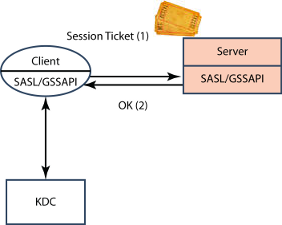
\includegraphics[height=2.5cm]{kerberos4.png}
\end{tabular}
\begin{tabular}{c}
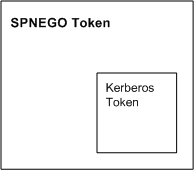
\includegraphics[height=2.5cm]{spnego.png}
\end{tabular}
\end{center}
\begin{enumerate}
\item Get a Kerberos service token
\item Wrap the token inside GSSAPI
\item Create a HTTP request filled with JSON records
\item Put the GSSAPI token inside the HTTP Negotiate header
\item Send the request to Apache
\end{enumerate}
{
\tiny \textbf{NOTE: The client connecting to Apache must already have a Kerberos ticket in its cache that is generated by calling \\ "kinit -k" or some other command. It does not use user/pass authentication.} 
}
\end{frame}

\begin{frame}[t, fragile]
\frametitle{Proxy configuration}
{ \tiny
\begin{center}
\begin{minipage}{.6\textwidth}
\begin{lstlisting}[basicstyle=\tiny,numberstyle=\tiny,backgroundcolor=\color{black!20}]
   <Proxy *>
      Order deny,allow
      Deny from all
      Allow from cern.ch
   </Proxy>
   <Location />
      #SSLRequireSSL
      AuthType Kerberos
      AuthName "CERN Login"
      KrbMethodNegotiate On
      KrbMethodK5Passwd Off
      KrbAuthRealms CERN.CH
      Krb5KeyTab /etc/krb5.keytab
      KrbVerifyKDC Off
      KrbServiceName host/lxfsrd0714.cern.ch@CERN.CH
      require valid-user
   </Location>
   ProxyPass / http://localhost:5984/ retry=0 nocanon
   ProxyPassReverse / http://localhost:5984/
   RequestHeader unset Authorization
\end{lstlisting}
\end{minipage}
\end{center}
}
\begin{itemize}
\item The keytab must be readable by the user running the httpd daemon
\item httpd must be enabled in SELinux
\end{itemize}
\end{frame}

\section{CouchDB}
\begin{frame}[c]
\begin{center}
\Huge \textcolor{BrickRed}{CouchDB}
\end{center}
\end{frame}

\begin{frame}[t]
\frametitle{Retrieving data}
\begin{itemize}
\item Any kind of query to CouchDB is represented as a view
\item There are two different kinds of views:
\begin{itemize}
	\item Permanent views - stored inside special design documents
	\item Temporary views - not stored in the database, but executed on demand
\end{itemize}
\item Permanent views are stored in CouchDB design documents whose id begins with \_design/ e.g. views for a blog are stored in \_design/blog
\end{itemize}
{
\tiny \textbf{NOTE: Temporary views are not adequate for production because they're very expensive to compute each time they're called} 
}
\begin{center}
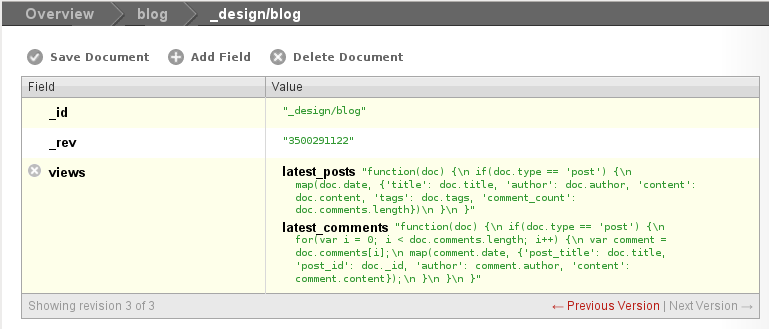
\includegraphics[height=4cm]{couchdb-view-big.png}
\end{center}
\end{frame}

\begin{frame}[t, fragile]
\frametitle{View functions}
\begin{itemize}
\item Each database in CouchDB can store multiple design documents
\begin{itemize}
	\item The views inside a design document are executed only for documents inside that particular database 
\end{itemize}
\item The view is defined by a mandatory JavaScript map function that maps keys to values
\end{itemize}
{ \tiny
\begin{center}
\begin{tabular}{c}
\begin{lstlisting}
function(doc) {
  emit(doc._id, doc);
}
\end{lstlisting}
\end{tabular}
\end{center}
\begin{center}
\begin{tabular}{c}
\begin{lstlisting}
function(doc) {
  if (doc.Type == "customer") {
    emit(doc.LastName, {FirstName: doc.FirstName, Address: doc.Address});
    emit(doc.FirstName, {LastName: doc.LastName, Address: doc.Address});
  }
}
\end{lstlisting}
\end{tabular}
\end{center}
}
\begin{itemize}

\item It is possible to use other languages than JavaScript by plugging in third-party view servers
\end{itemize}
\end{frame}

\begin{frame}[t, fragile]
\frametitle{map/reduce}
\begin{itemize}
\item If a view has the optional reduce function, it is used to produce aggregate results for that view
\end{itemize}
{ \tiny
\begin{center}
\begin{tabular}{c}
\begin{lstlisting}
function(doc) {
  emit(doc.machine, doc.cputime);
}
\end{lstlisting}
\end{tabular}
\begin{tabular}{c}
\begin{lstlisting}
function (key, values) {
    return sum(values);
}
\end{lstlisting}
\end{tabular}
\end{center}
\begin{itemize}
\normalsize \item Keys can be grouped (group=true)
\begin{itemize}
	\item Reduce function summarizes values of rows that share the same key
\end{itemize}
\end{itemize}
\begin{center}
\begin{tabular}{|c|c|}
	\hline
	\textbf{key} & \textbf{value} \\
	\hline
	\hline
	"spock.cern.ch" & 2 \\
	\hline
	"kirk.cern.ch" & 4 \\
	\hline
	"spock.cern.ch" & 7 \\
	\hline
	"picard.cern.ch" & 8 \\
	\hline
\end{tabular}
\begin{tabular}{c}
	$\Longrightarrow$ \\
\end{tabular}
\begin{tabular}{|c|c|}
	\hline
	\textbf{key} & \textbf{value} \\
	\hline
	\hline
	"spock.cern.ch" & 9 \\
	\hline
	"kirk.cern.ch" & 4 \\
	\hline
	"picard.cern.ch" & 8 \\
	\hline
\end{tabular}
\end{center}
}
\begin{itemize}
\item Reducing and it's grouping mechanism can be set to false
\begin{itemize}
	\item Without grouping the reduce function above does nothing
\end{itemize}
\end{itemize}
\end{frame}

\begin{frame}[t, fragile]
\frametitle{Documents}
{
\tiny
\begin{center}
\Ovalbox{sysacct-records}
\Ovalbox{sysacct-summaries}
\Ovalbox{
\begin{tabular}{c}
\pause
\begin{lstlisting}
{
   "UserID": {
       "LocalUserId": "smmsp"
   },
   "ProbeName": "lxfsrd0714.cern.ch",
   "Grid": "CERN",
   "RecordData": [
       {
           "JobName": "sendmail",
           "StartTime": "1314360061.0",
           "Memory": "57696.0",
           "WallDuration": "0.08",
           "CpuDuration": "0.01",
           "EndTime": "1314360061.08"
       }
   ]
}
\end{lstlisting}
\pause
\begin{lstlisting}
{
   "UserID": {
       "LocalUserId": "root"
   },
   "ProbeName": "lxfsrd0714.cern.ch",
   "Grid": "CERN",
   "RecordData": [
       {
           "JobName": "Summary",
           "StartTime": "1314356165.0",
           "Memory": "17841.5258437",
           "WallDuration": "14562.38",
           "CpuDuration": "1.41",
           "EndTime": "1314361082.8"
       }
   ]
}
\end{lstlisting}
\end{tabular}{c}
}
\end{center}
}
\begin{itemize}
\pause \item Two databases:
\begin{itemize}
	\item sysacct\_records - detailed information about commands
	\item sysacct\_summaries - summarized information after each collection
\end{itemize}
\end{itemize}
\end{frame}

\begin{frame}[t]
\frametitle{Queries}
\begin{itemize}
\item Some of the basic questions the queries should answer:
\begin{enumerate}
	\pause \item Which commands did a user execute?
	\pause \item On which machines was he/she active?
	\pause \item What time was he/she active?
	\pause \item Where was this command executed, by whom and at what time?
	\pause \item What is the first and last time a user was active on a machine?
	\pause \item What time did he/she execute a command on a machine?
\end{enumerate}
\pause \item Some of the queries (2,3,5) can be done on both summaries or records, some (1,4,6) only on records
\begin{itemize}
	\item Command names
	\item Activity time range
\end{itemize}
\item Any kind of query that requires information for individual commands has to use the record documents
\end{itemize}
\end{frame}

\begin{frame}[t, fragile]
\frametitle{Views}
\begin{itemize}
\item Let's start with number 2
\end{itemize}
{ \tiny
\begin{center}
\begin{tabular}{c}
\begin{lstlisting}[language=Python]
# User was active on machines X,Y,Z... (summaries)

def fun(doc):
  for record in doc["RecordData"]:
    yield [doc["UserID"]["LocalUserId"], doc["ProbeName"]], None

def fun(keys, values):
  return None

\end{lstlisting}
\end{tabular}
\end{center}
}
\begin{itemize}
\pause \item Q: Why do we need the reduce function?
\pause \item Summaries are generated for a user on a machine at 10pm, 11pm...
\begin{itemize}
	\item The view is called for every document in the database
	\item yield generates keys for every document (keys are not unique)
\end{itemize}
\pause \item A: For grouping
\end{itemize}
{ \tiny
\begin{center}
\begin{tabular}{|l|l|}
	\hline
	\textbf{key} & \textbf{value} \\
	\hline
	\hline
	["root", "spock.cern.ch"] & null \\
	\hline
	["root", "kirk.cern.ch"] & null \\
	\hline
	["root", "spock.cern.ch"] & null \\
	\hline
	["smmsp", "spock.cern.ch"] & null \\
	\hline
\end{tabular}
\pause
\begin{tabular}{c}
	$\Longrightarrow$ \\
\end{tabular}
\begin{tabular}{|l|l|}
	\hline
	\textbf{key} & \textbf{value} \\
	\hline
	\hline
	["root", "spock.cern.ch"] & null \\
	\hline
	["root", "kirk.cern.ch"] & null \\
	\hline
	["smmsp", "spock.cern.ch"] & null \\
	\hline
\end{tabular}
\end{center}
}
\end{frame}

\begin{frame}[t, fragile]
\frametitle{Time ranges}
\begin{itemize}
\item Where was this command executed, by whom and at what time?
\begin{itemize}
	\item Not nearly as easy to figure out as it seems
\end{itemize}
\item If we want to get information for a particular command:
\begin{itemize}
	\item The command name has to be the first part of the key so it can be searched
\end{itemize}
\end{itemize}
{ \tiny
\begin{center}
\begin{tabular}{c}
\begin{lstlisting}[language=Python]
# Command was executed by user X on machine Y at time Z (records)
# View: commands/exectimes
def fun(doc):
  if doc["ProbeName"] and doc["RecordData"] and doc["UserID"]:
    for command in doc["RecordData"]:
      yield [command["JobName"],doc["UserID"]["LocalUserId"],doc["ProbeName"], command["StartTime"]]
\end{lstlisting}
\end{tabular}
\end{center}
}
\begin{itemize}
\pause \item Again, there will be duplicate keys
\pause \item Should we group to get unique keys?
\pause \item Is it better to have larger values or more keys?
\begin{itemize}
	\item Should the timestamps be part of the key or values?
\end{itemize}
\end{itemize}
\end{frame}

\begin{frame}[t, fragile]
\frametitle{DB output}
\begin{itemize}
\item "Grow tall, not wide"
\begin{itemize}
	\item Reduce function should only be used to get a smaller number of values
\end{itemize}
\item This is slow and inefficient:
\end{itemize}
{ \tiny
\begin{center}
\begin{tabular}{c}
\begin{lstlisting}[language=Python]
# Command was executed by user X on machine Y at time Z (records)
# View: commands/exectimes
def fun(doc):
  if doc["ProbeName"] and doc["RecordData"] and doc["UserID"]:
    for command in doc["RecordData"]:
      yield [command["JobName"],doc["UserID"]["LocalUserId"],doc["ProbeName"]], 
      		command["StartTime"]
      		
def fun(keys, values):
  return values
\end{lstlisting}
\end{tabular}
\end{center}
}
\begin{itemize}
\pause \item Option: get all the keys and format output by external scripts
\end{itemize}
\end{frame}
\begin{frame}[t, fragile]
\frametitle{Searches}
\begin{itemize}
\item Row keys are sorted
\end{itemize}
{ \tiny
\begin{center}
\begin{tabular}{|l|l|}
	\hline
	\textbf{key} & \textbf{value} \\
	\hline
	\hline
	["sendmail", "ssmp", "spock.cern.ch", "1333333333"] & null \\
	\hline
	["sh", "root", "kirk.cern.ch", "1333333334"] & null \\
	\hline
	["sh", "root", "spock.cern.ch", "1333333335"] & null \\
	\hline
\end{tabular}
\end{center}
}
\begin{itemize}
\pause \item How would we search for the command sh?
\end{itemize}
\pause
{ \tiny
\begin{center}
\begin{verbatim}
$ curl -X GET 'http://localhost:5984/sysacct_records/_design/commands/_view/exectimes
					?startkey=\["sh"\]&endkey=\["sh", \{\}]'
\end{verbatim}
\end{center}
}
\begin{itemize}
\pause
\item This will get us all the keys with "sh"
\item For further filtering additional help is needed
\pause
\begin{itemize}
	\item A Python script that iterates through every key and creates a dictionary
	\item Or we could use Bash directly with curl...
\end{itemize}
\end{itemize}
\end{frame}

\begin{frame}[t, fragile]
\frametitle{Local processing}
\begin{itemize}
\item Questions arise:
\begin{itemize}
\pause	\item Is it better to give more work to the script or the database?
\pause	\item Should the script get a smaller/larger number of non-unique keys?
\pause	\item How should the final output be formatted?
\end{itemize}
\pause \item Guideline:
\begin{itemize}
	\item Database will always have a high load, query scripts on desktop computers should do as much work as possible
\end{itemize}
\pause \item Calculated decisions (could be the wrong ones):
\begin{itemize}
\pause	\item Make the queries as specific as possible (don't get everything!)
\pause	\item Choose more keys per value over less values per key (parse it later)
\pause	\item Avoid using reduce functions only for grouping (do it in the script)
\end{itemize}
\pause \item Retrieval+presentation of data is achieved by a combination of views inside the database and scripts that call the views
\end{itemize}
\end{frame}

\begin{frame}[t, fragile]
\frametitle{Indexing}
\begin{itemize}
\item The first time a view is executed CouchDB indexes results in a B-tree
\begin{itemize}
	\item It can take a long time for the first call to return results
	\item Subsequent calls are much faster because a B-tree exists
\end{itemize}
\item Our views are going to be rarely executed
\begin{itemize}
	\item We can update our B-tree periodically (warm up the views)
\end{itemize}
\end{itemize}
{ \tiny
\begin{center}
\begin{tabular}{c}
\begin{lstlisting}[language=Python, escapechar=!]]
class ViewUpdater(object):
!\pause!    # The smallest amount of changed documents before the views are updated
    MIN_NUM_OF_CHANGED_DOCS = 50
    
    # Set the minimum pause between calls to the database
    PAUSE = 5 # seconds
    
    # URL to the DB on the CouchDB server
    URL = "http://localhost:5984"
    
!\pause!    # One entry for each design document 
    # in each database
    VIEWS = {
        'sysacct_records': {
            'commands': [
                'exectimes',
                # ...
            ]
        }
    }
\end{lstlisting}
\end{tabular}
\end{center}
}
\end{frame}

\section*{}
\begin{frame}[t]
\frametitle{Conclusion}
\begin{itemize}
\item Most NoSQL databases have no security
\item Debian distributions use a different psacct format
\item Python documentation for Kerberos is obscure
\item Reduce functions should reduce
\item Grow tall not wide
\item Views written in JavaScript are the fastest
\item Views should be prewarmed
\item Design documents should have less views
\item Collector can be expanded to collect other data
\item NoSQL databases require a very different approach
\end{itemize}
\end{frame}

\begin{frame}
\begin{center}
\LARGE \textcolor{red}{Questions?}
\end{center}
\end{frame}
\end{document}
